Software guards our secrets, our money, our intellectual property,
our reputation \cite{covern}.  We entrust personal and
corporate information to software which works in an \emph{open} world, 
where  it interacts with % a vast number of
third party software of unknown provenance, possibly buggy and potentially malicious.

Thus, we expect and hope that our software will be \emph{robust}:
We expect and hope our software to behave correctly even if  used 
by erroneous or malicious third parties. Robustness means 
something different for different software.\susan{I put in the ERC20 citation but I don't see what that has to do with banks authorising payments}
 We expect that our bank will only make payments 
from our account if instructed by us or somebody authorized\cite{ ERC20}, 
and that  space on a web given to an advertiser will not be used
to obtain access to our bank details\cite{cwe}. 

The importance of robustness has lead to the design of many programming
language mechanisms which help write robust programs:
constant fields or methods, private methods/fields, ownership\cite{ownalias}
as well as the object capability paradigm\cite{MillerPhD},
and its adoption in  web systems
\cite{CapJavaHayesAPLAS17,CapNetSocc17Eide,DOCaT14} and programming languages such as Newspeak
\cite{newspeak17}, Dart \cite{dart15}, Grace \cite{grace,graceClasses}, Wyvern \cite{wyverncapabilities}.

While such programming language mechanisms make it \textit{possible} to write robust
programs, they cannot \textit{ensure} that programs are robust. 
To be able to do this, we need ways to specify what robustness means for the 
particular program, and ways to demonstrate that the particular program 
adheres to its specific robustness requirements.

There has been a plethora of work on the specification and verification of the
functional correctness of programs. Such specifications describe what are
essentially \emph{sufficient} conditions for some
effect to happen. For example, if you make a payment request to your bank, money will be transferred
and as a result your funds will be reduced: the payment request is a sufficient condition for the
reduction of funds. However, a bank client is also interested in \emph{necessary} conditions:
they want to be assured that no reduction in their funds will take place unless they themselves
requested it.

Necessary conditions are essentially about things that will  \emph{not} happen. For example,
there  will be no reduction to the account's funds without the owner's explicit request: the request being made by
the owner is the necessary condition - under no other circumstances will the funds be reduced.

We give a visual representation of the difference between sufficient and necessary conditions in 
Fig. \ref{fig:NecessaryAndSuff}. We
represent the space of all theoretically possible behaviours as points in the rectangle, 
each function is a coloured oval and its possible behaviours are the points in the area of that oval.  
The sufficient conditions are described on a per-function basis. 
The necessary conditions, on the other hand are about the behaviour of a module as a whole, 
and describe what is guaranteed not to happen;
they are depicted as black triangles.
\susan{shouldn't some of the black triangles overlap the ovals? Otherwise they are not restricting any behavours}

  \begin{figure}[htb]
 \begin{tabular}{ccccc}
\begin{minipage}{0.25\textwidth}
 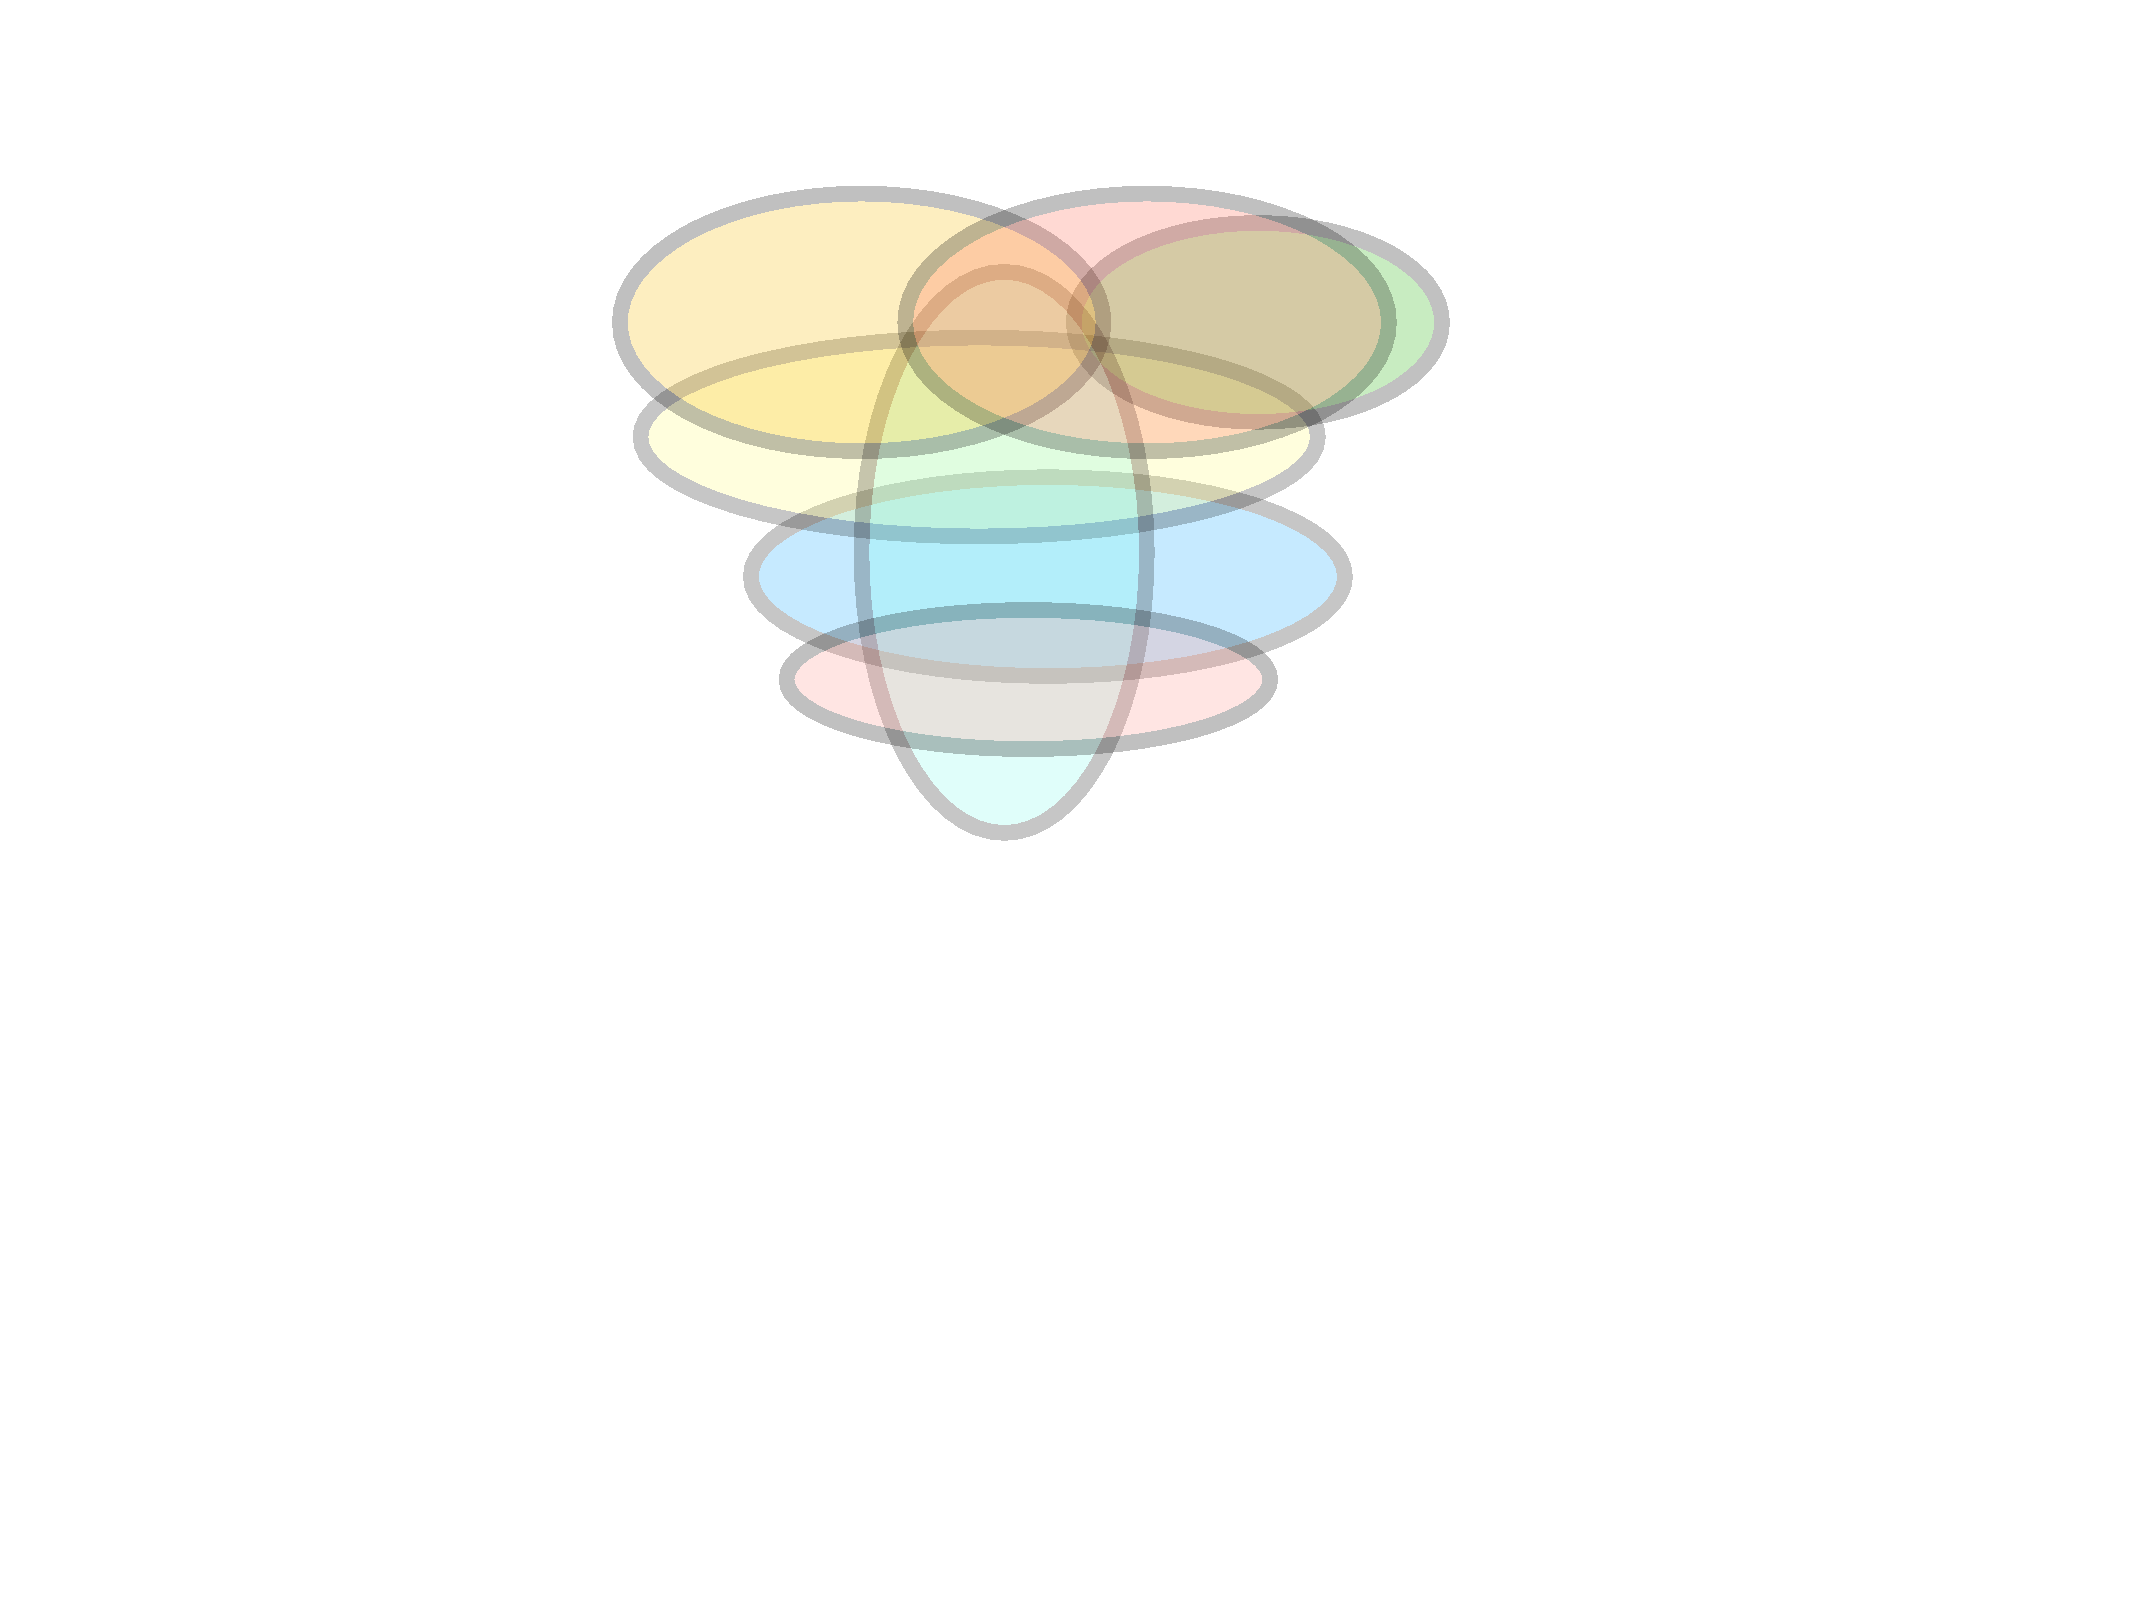
\includegraphics[width=\linewidth, trim=250  320 260 60,clip]{diagrams/Suff.pdf}
\end{minipage}
 & \ \ \ & 
\begin{minipage}{0.25\textwidth}
 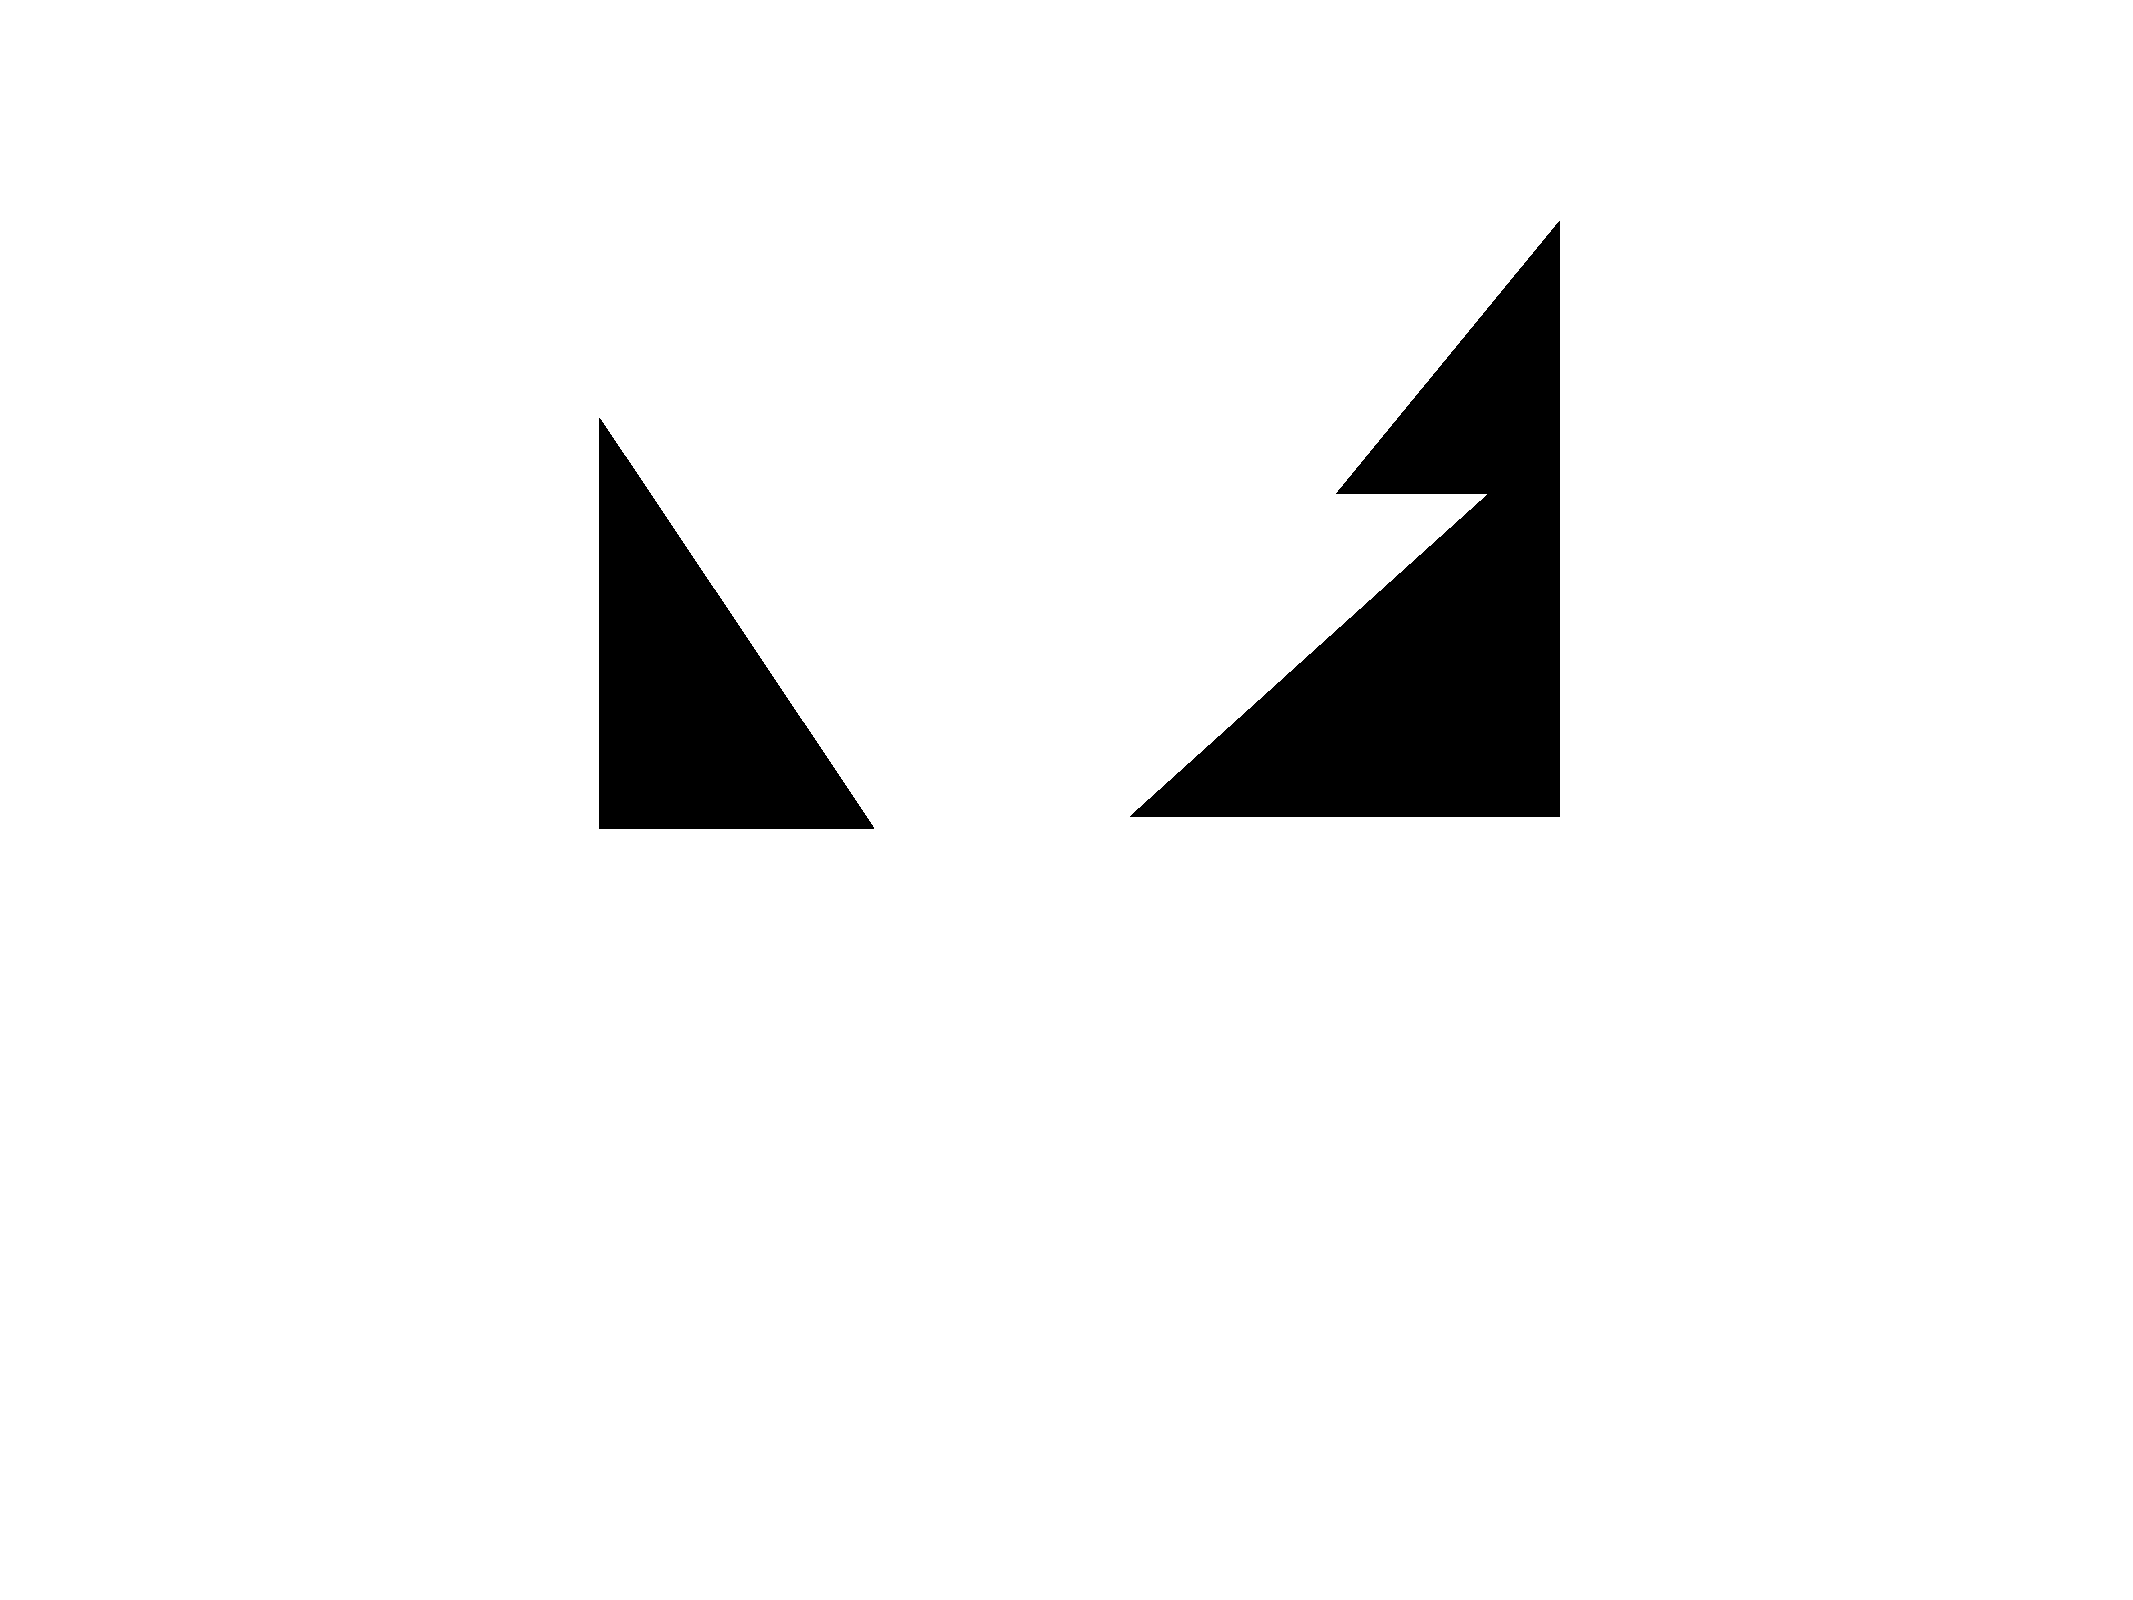
\includegraphics[width=\linewidth, trim=250  320 260 60,clip]{diagrams/Nec.pdf}
\end{minipage}
 & \ \ \ &
\begin{minipage}{0.25\textwidth}
 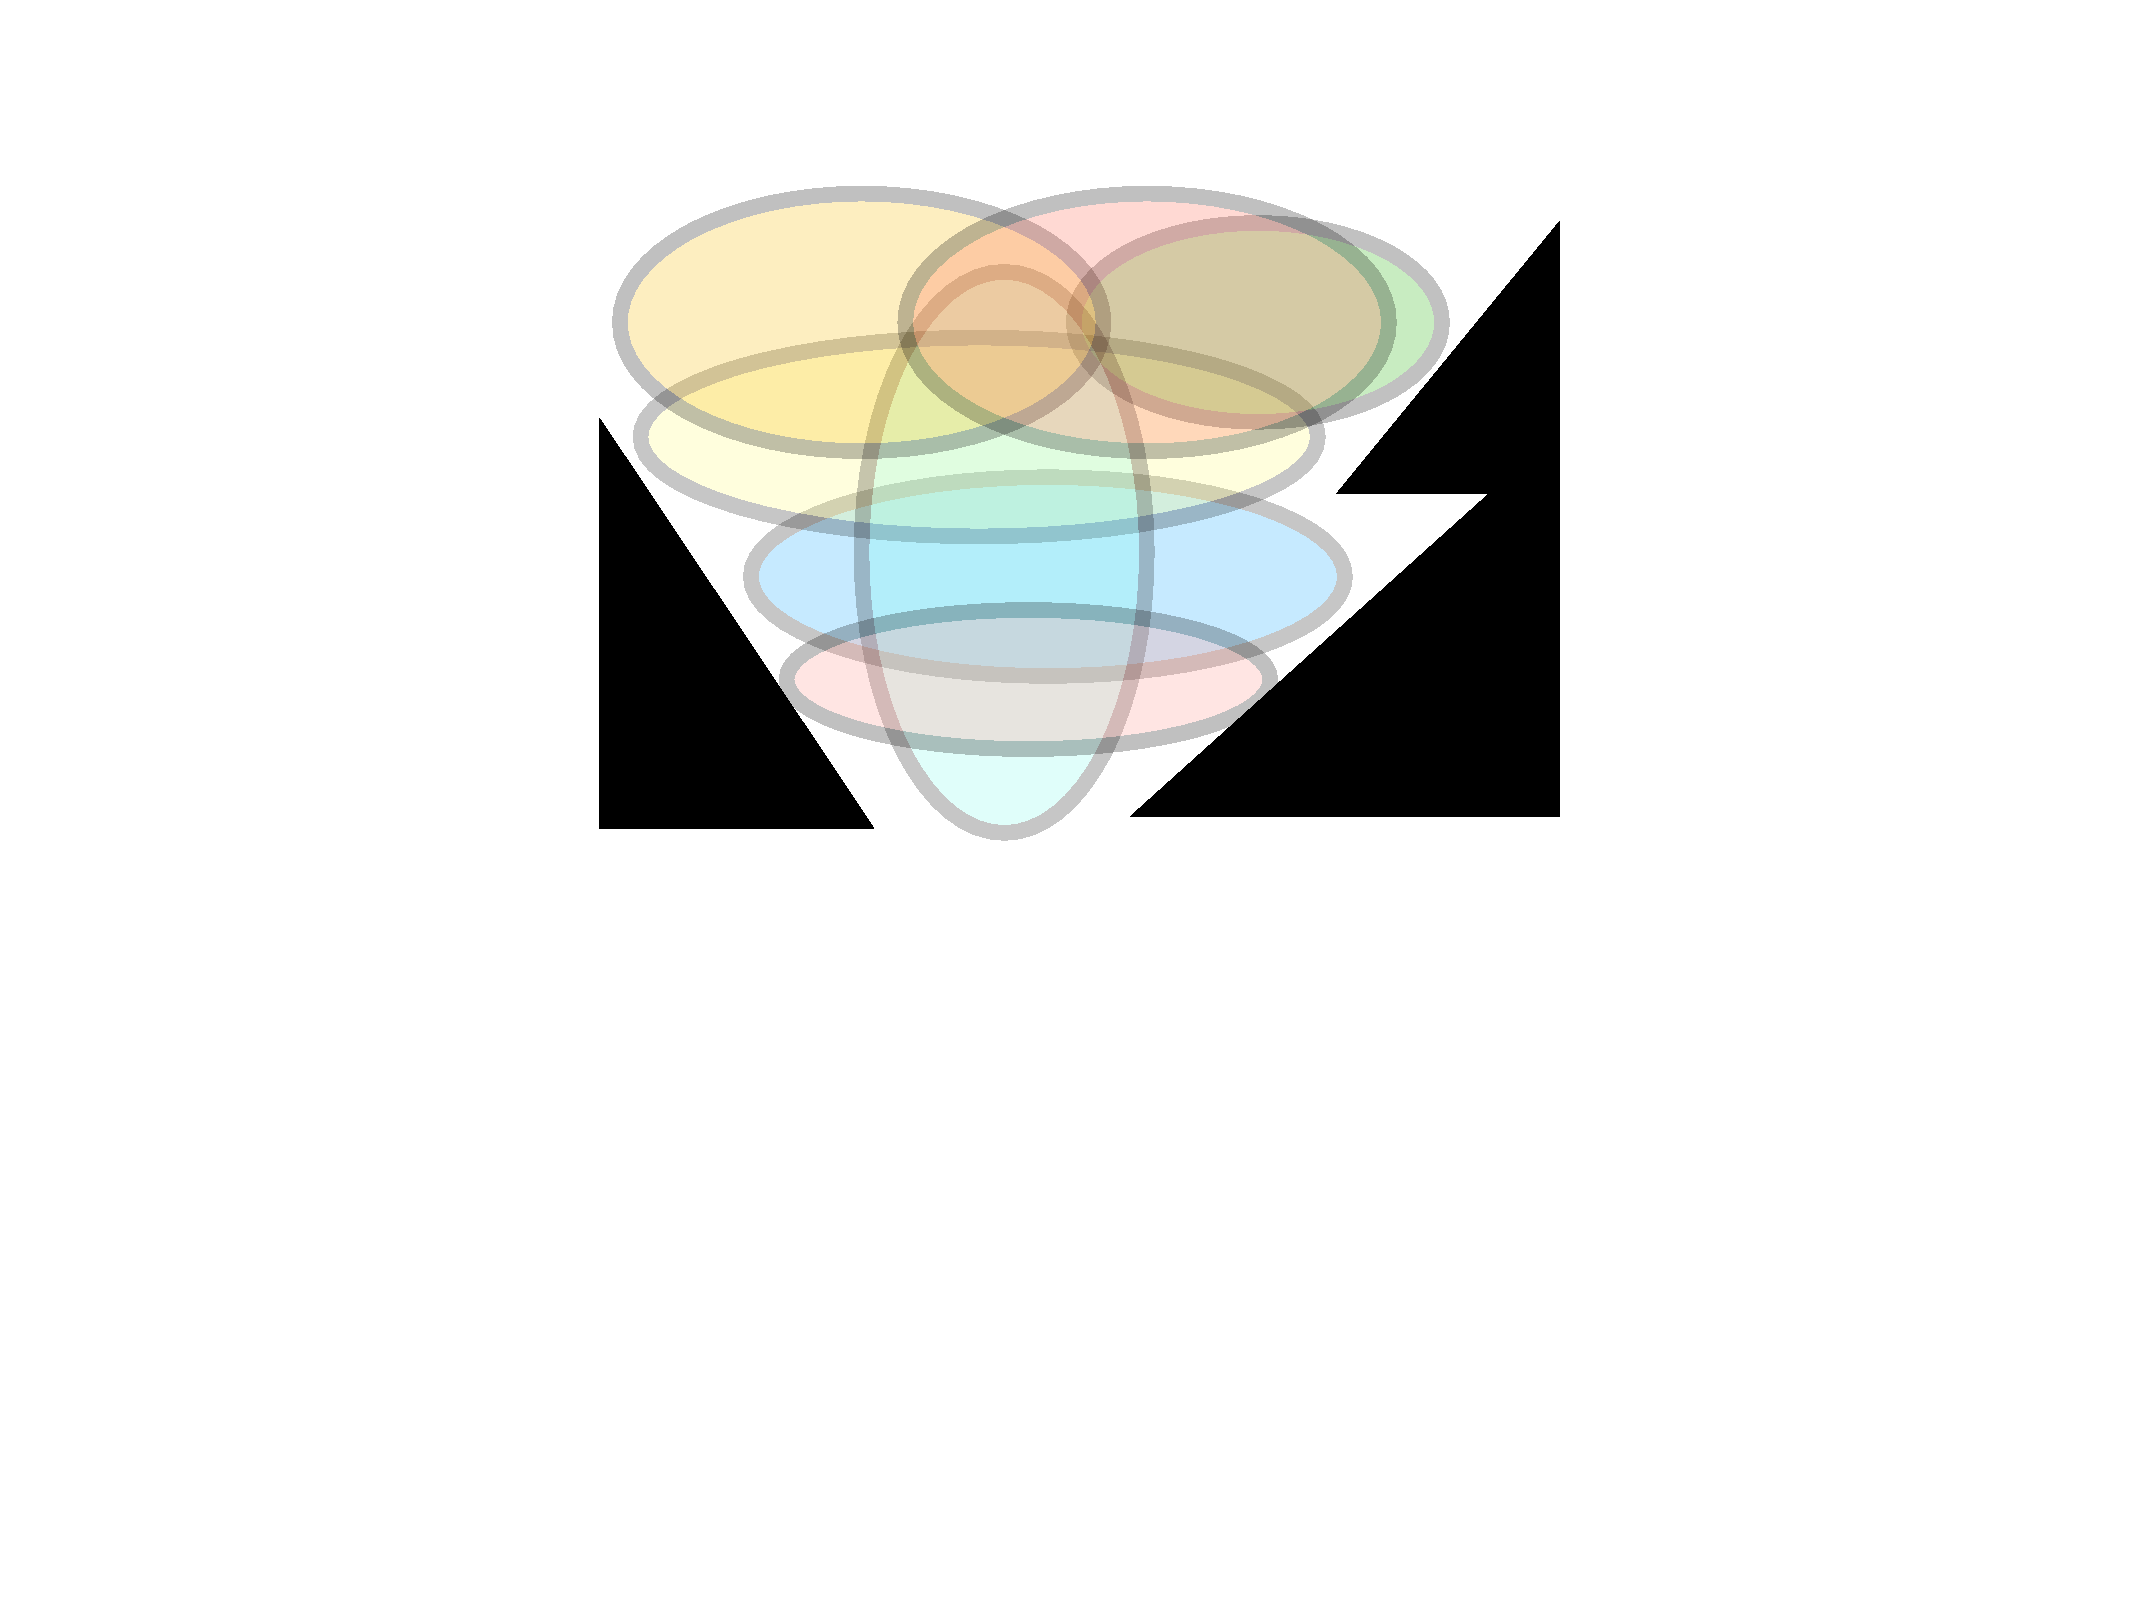
\includegraphics[width=\linewidth, trim=250  320 260 60,clip]{diagrams/NecAndSuff.pdf}
\end{minipage}
\\
sufficient  spec.& & necessary spec. & & holistic spec.
%\begin{minipage}{0.75\textwidth}
%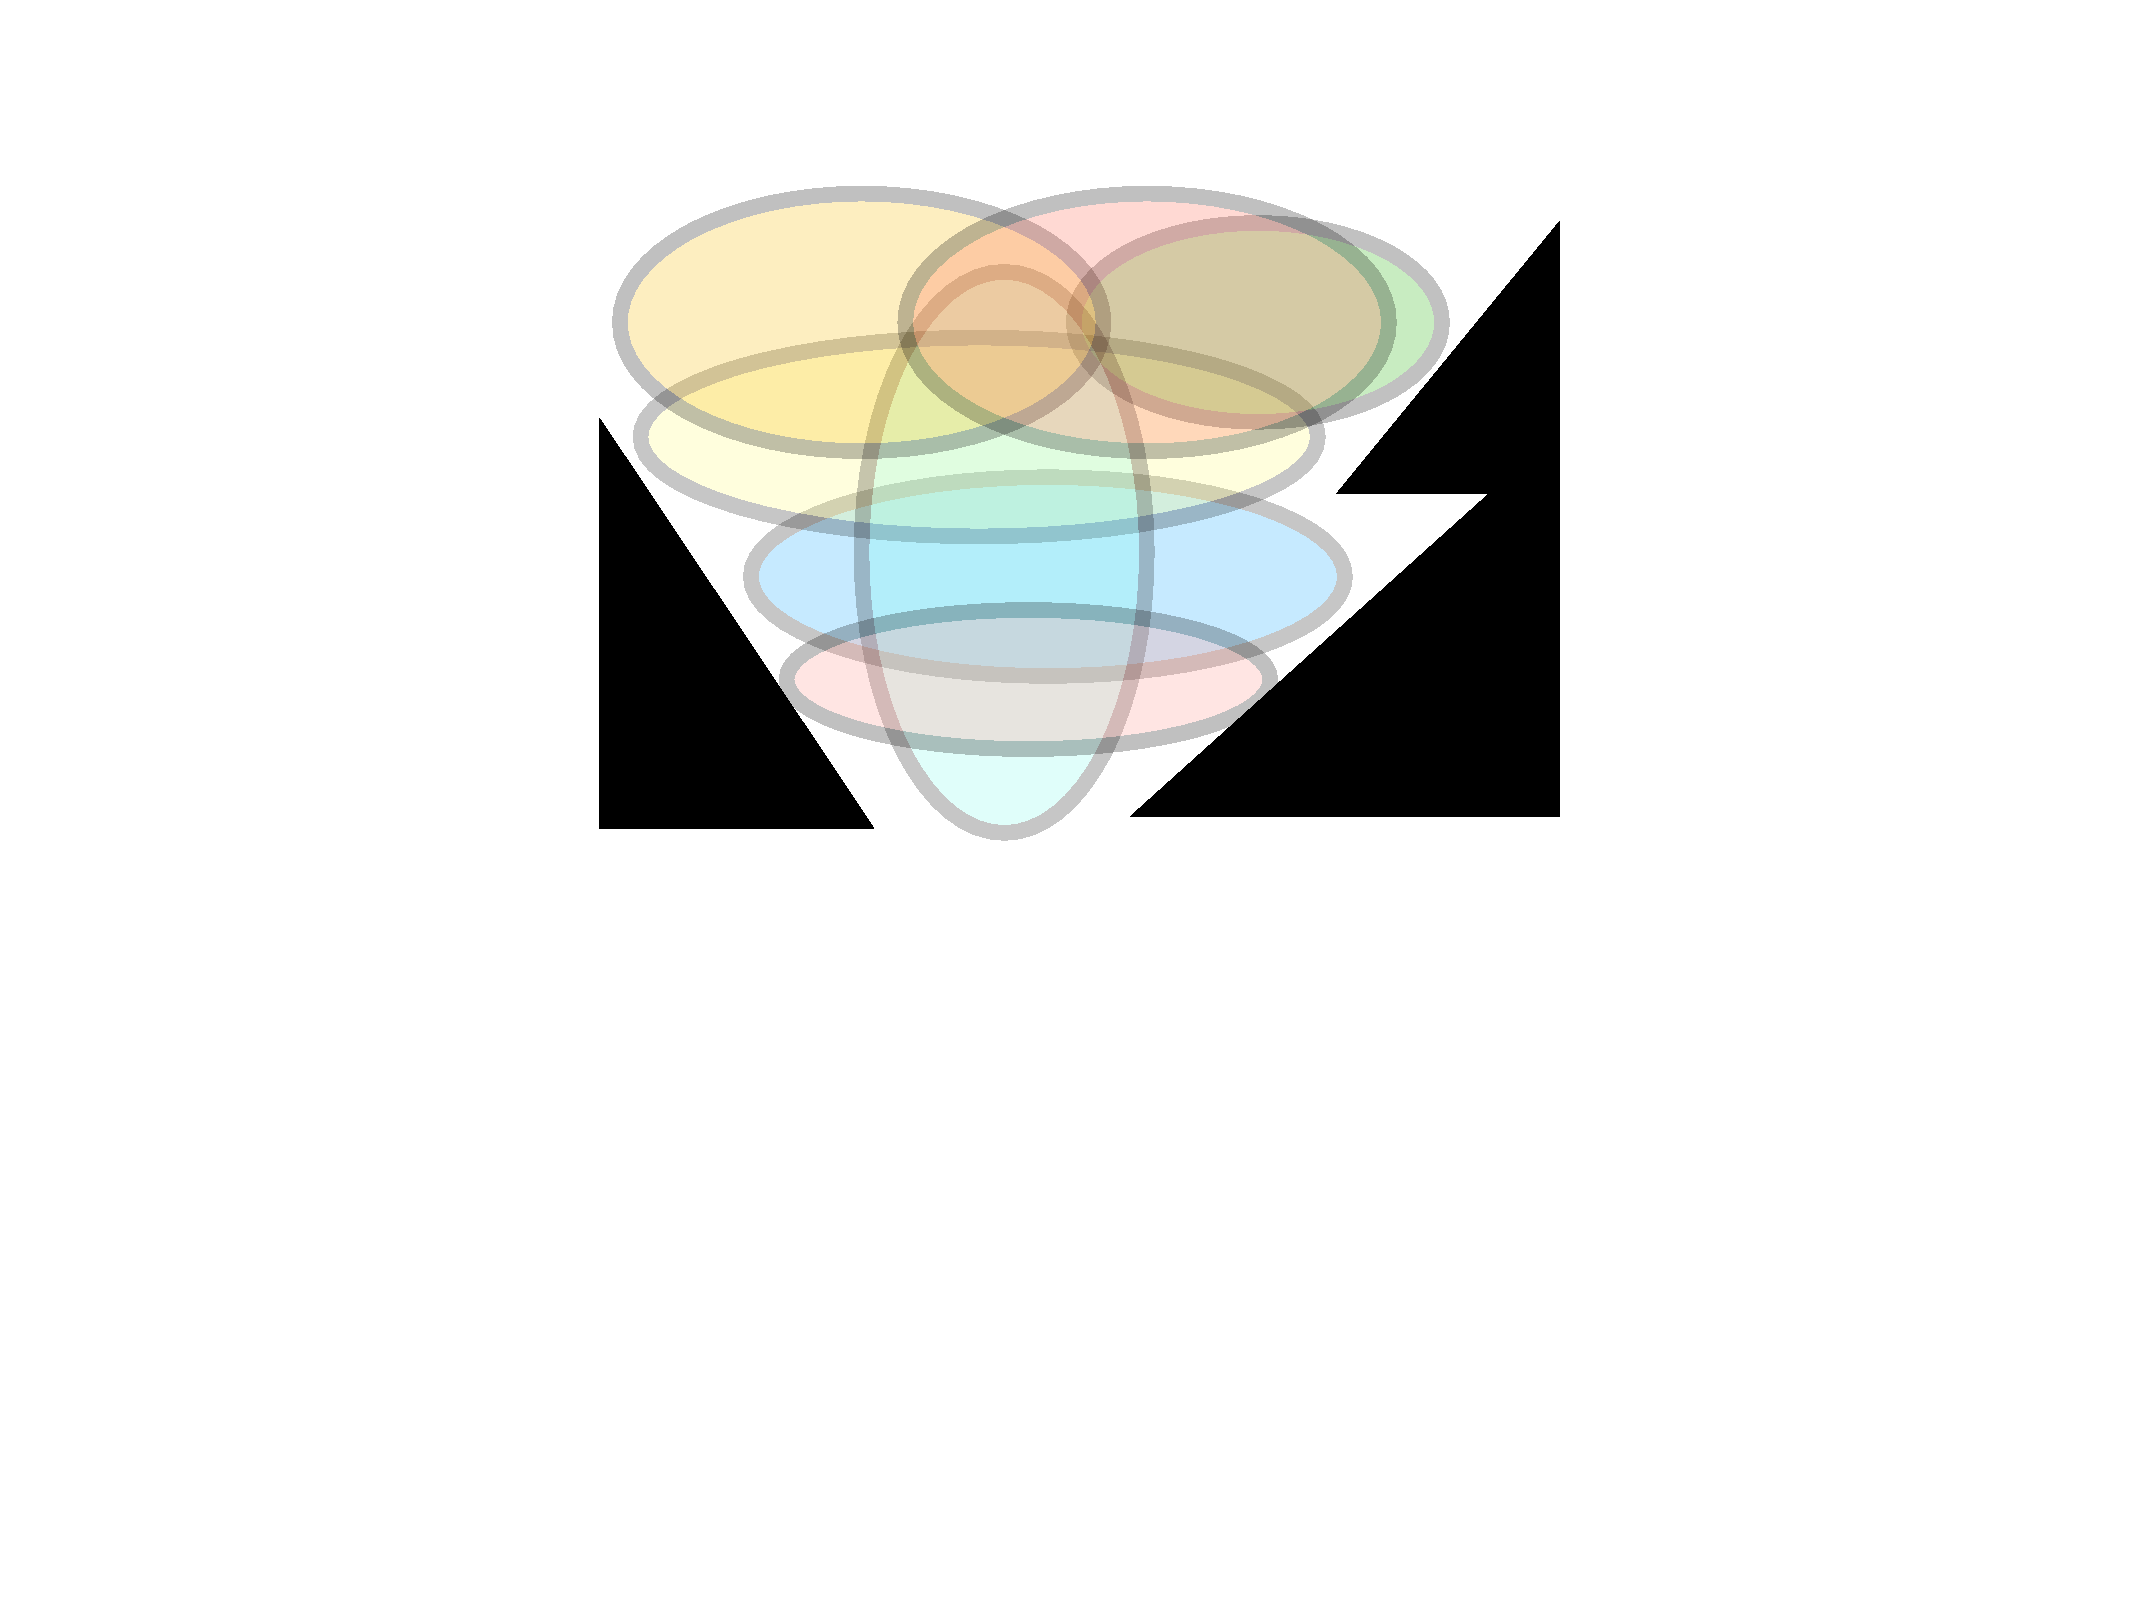
\includegraphics[width=\linewidth, trim=145  320 60 105,clip]{diagrams/NecAndSuff.pdf}
%\end{minipage}
%% y seems to eat up the bollom
%% x eats space from left, if you increase it the diagram decreases from left
%% w eats space from top, if you increase it the diagram decreases from top
%%\includegraphics[page=3, width=\linewidth, trim=150  270 40 150, clip]{diagrams/snmalloc.pdf}
%\sdcomment\sophia{I think we need to change the diagram so that it says small slab.}
%\end{minipage}
 \end{tabular}
  \vspace*{-2.5mm}
  \caption{Sufficient and Necessary Conditions, and Full Specifications}
 \label{fig:NecessaryAndSuff}
 \end{figure}
 
 We propose that  necessary conditions should be explicitly stated. Specifications should be \emph{holistic}, in the sense that they describe the  overall behaviour of a module: not only the behaviour of each of its functions separately, but also 
 emerging behaviours through combination of functions.
% Necessary conditions are  depicted by the black
% triangles in the middle  diagram in Fig \ref{fig:NecessaryAndSuff}.
A holistic specification should therefore consist of   the sufficient as well as the necessary conditions, as  
depicted in right hand side  diagram in Fig. \ref{fig:NecessaryAndSuff}.
In Section \ref{sec:discussion} we argue why necessary conditions are more than the complement of
sufficient conditions.

Necessary conditions are guarantees upheld throughout program execution.
Other systems which give such ``permanent'' guarantees are  type systems, 
\susan{I would stop after the first sentence - the other points perhaps in related work}
which ensure that well-formed programs  always produce well-formed runtime
configurations, or information flow control systems \cite{infoflow}, which ensure that values 
classified as high  will not be passed into contexts classified as low. 
Such  guarantees %made by types or information flow control
 are  practical to check, but   too coarse grained
for the purpose of fine-grained,  module-specific specifications. 

Necessary conditions are  akin to monitor or object invariants\cite{Hoare74,Meyer97}. The difference between
these and our holistic specifications is that object/monitor invariants can only reflect  on
the current state (\ie the contents of the
stack frame and the heap), while  holistic specifications reflect on all aspects of execution.

In this paper we propose \Chainmail, a specification language to express holistic specifications. \Chainmail extends 
traditional program specification languages\cite{Leavens-etal07,Meyer92}, with features which talk about:

\susan{These features sort of come from nowhere, so I wonder whether we even want them in the introduction. I think if you do then something more about open systems, (that what is critical is controlling access from foreign code and that you need to be able to talk about that in the specification language) should come first.}
\begin{description}
\item[Permission] Which object may have access to which other objects. 
Accessibility is central since access to an object usually also grants access to the functions it provides.

\item[Control] What object called functions on other objects. This is useful in identifying the causes of certain effects - eg 
funds can only be reduced if the owner called a payment function.

\item[Authority]  Which objects' state or properties may change. This is useful in describing effects, such as reduction of funds.

\item[Space] This is about which parts of the heap are considered when establishing some property, or when 
performing program execution and is
related to, but different from memory footprints and separation logics.

\item[Time] Assertions about the past or the future.
\end{description}

The design of \Chainmail was guided by the study of a sequence of examples from the OCAP literature and the 
smart contracts world: the membrane, the DOM, the Mint/Purse, the Escrow, the DAO and ERC20. 
We were satisfied to see that the same concepts were used to specify examples from  different contexts.
Holistic assertions often have the form of a guarantee
 that if some property ever hods in the future then some other property holds now.
For example, if within a certain heap some change is possible in the future, then this particular heap contains 
at least one object which has access to a specific other, privileged object.
%
While many individual features of \Chainmail can be found also in other work, 
we argue that their power and novelty for specifying open systems lies in their careful combination.
%\sdcomment
\sophia{ I think that James does not like this sentence. What could we say instead? Also, we need to
stress that the selection of these features was not arbitrary.}
 
A module satisfies such a holistic assertion if, for all other modules,
  the assertion is satisfied  in all runtime configurations reachable through execution of the two modules combined.
  This reflects the open-world view.
  
The contributions of this paper are:
\begin{itemize}
\item the design of the holistic specification language \Chainmail,
\item the semantics of \Chainmail,
\item a validation of \Chainmail through its application to a sequence of examples,
\item a further validation of \Chainmail through informal proofs of adherence of code to some of these specifications.
\end{itemize}  
  
  
The rest of the paper is organized as follows: Section~\ref{sect:motivate:Bank} 
motivates our work in terms of an example. Sections~\ref{sect:LangOO} contain a formal definition of \LangOO, and Section~\ref{sect:assertions} the semantics of assertions. Section ... related work .... Section xxxx concludes.

